\subsubsection{IPv6 auto Adresse}
\begin{figure}[!htb]
    \centering
    \begin{subfigure}{\textwidth}
        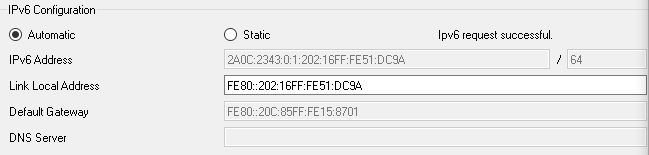
\includegraphics[width=\textwidth,height=\textwidth,keepaspectratio]{./img/user1.png}
        \caption{User 1}
    \end{subfigure}
    \begin{subfigure}{\textwidth}
        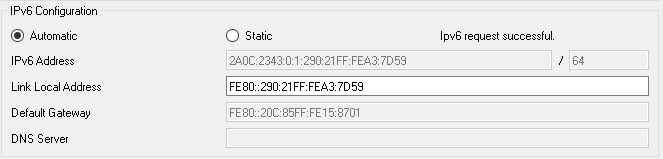
\includegraphics[width=\textwidth,height=\textwidth,keepaspectratio]{./img/user2.png}
        \caption{User 2}
    \end{subfigure}
    \begin{subfigure}{\textwidth}
        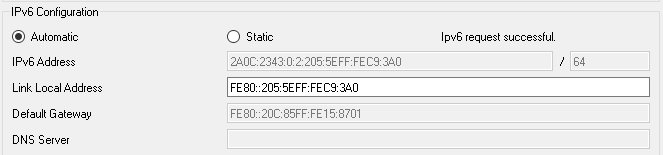
\includegraphics[width=\textwidth,height=\textwidth,keepaspectratio]{./img/admin1.png}
        \caption{Admins 1}
    \end{subfigure}
    \begin{subfigure}{\textwidth}
        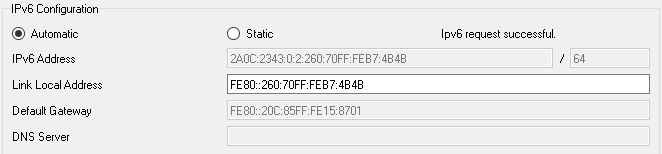
\includegraphics[width=\textwidth,height=\textwidth,keepaspectratio]{./img/admin2.png}
        \caption{Admin 2}
    \end{subfigure}
    \caption{Auto IPv6 an den Endsystemen}
\end{figure}
\subsubsection{Ping Test}
\begin{figure}[!htb]
    \centering
    \begin{subfigure}{.8\textwidth}
        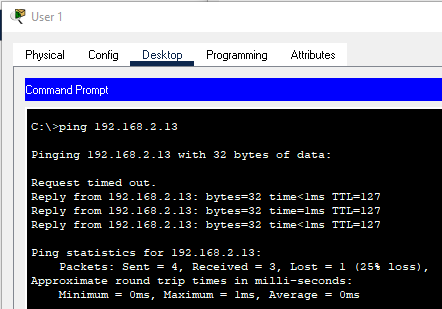
\includegraphics[width=\textwidth,height=.85\textwidth,keepaspectratio]{./img/user_ping_admin.png}
        \caption{IPv4}
    \end{subfigure}
    \begin{subfigure}{.8\textwidth}
        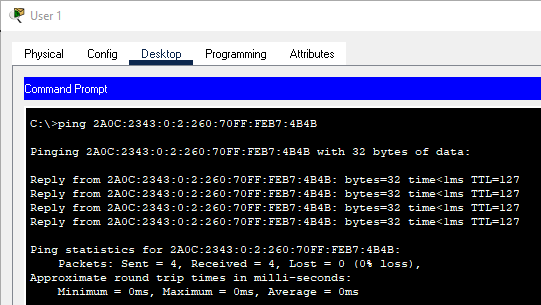
\includegraphics[width=\textwidth,height=.85\textwidth,keepaspectratio]{./img/ipv6_user_ping_admin.png}
        \caption{IPv6}
    \end{subfigure}
    \caption{Ping von User zu Admin}
\end{figure}
\FloatBarrier
\subsubsection{Frage 2}
\paragraph{Frage}
Warum funktioniert die Autokonfiguration bei IPv6 ohne Erstellung eines
DHCP Services, und worin besteht der Unterschied zu DHCPv6?
\paragraph{Antwort}
Weil IPv6 automatisch SLAAC nutzt und die Adresse einfach ohne Vergleiche ausgewählt wird. IPv6 wurde so designt, dass man keinen DHCP Server benötigt. Wenn die Adresse nach der Zuweisung doch vorhanden sein sollte, wird eine neue vergeben.
Bei (Stateful) DHCPv6 gibt es einen DHCP Server der alles zuweist und auch gleich die richtige Adresse den Host gibt. Hier können zb. Adressen ausgeschlossen werden, was bei SLAAC nicht geht.